\chapter{Kodea}.

Kodeari buruzko hainbat ohar emateko.

\section{Gauss metodoa}
\label{sec:B1}

\subsection*{Metodoaren koefizienteak.}
GaussCollocationCoefficients.nb funtzioa.

\begin{figure}[h!]
\centerline{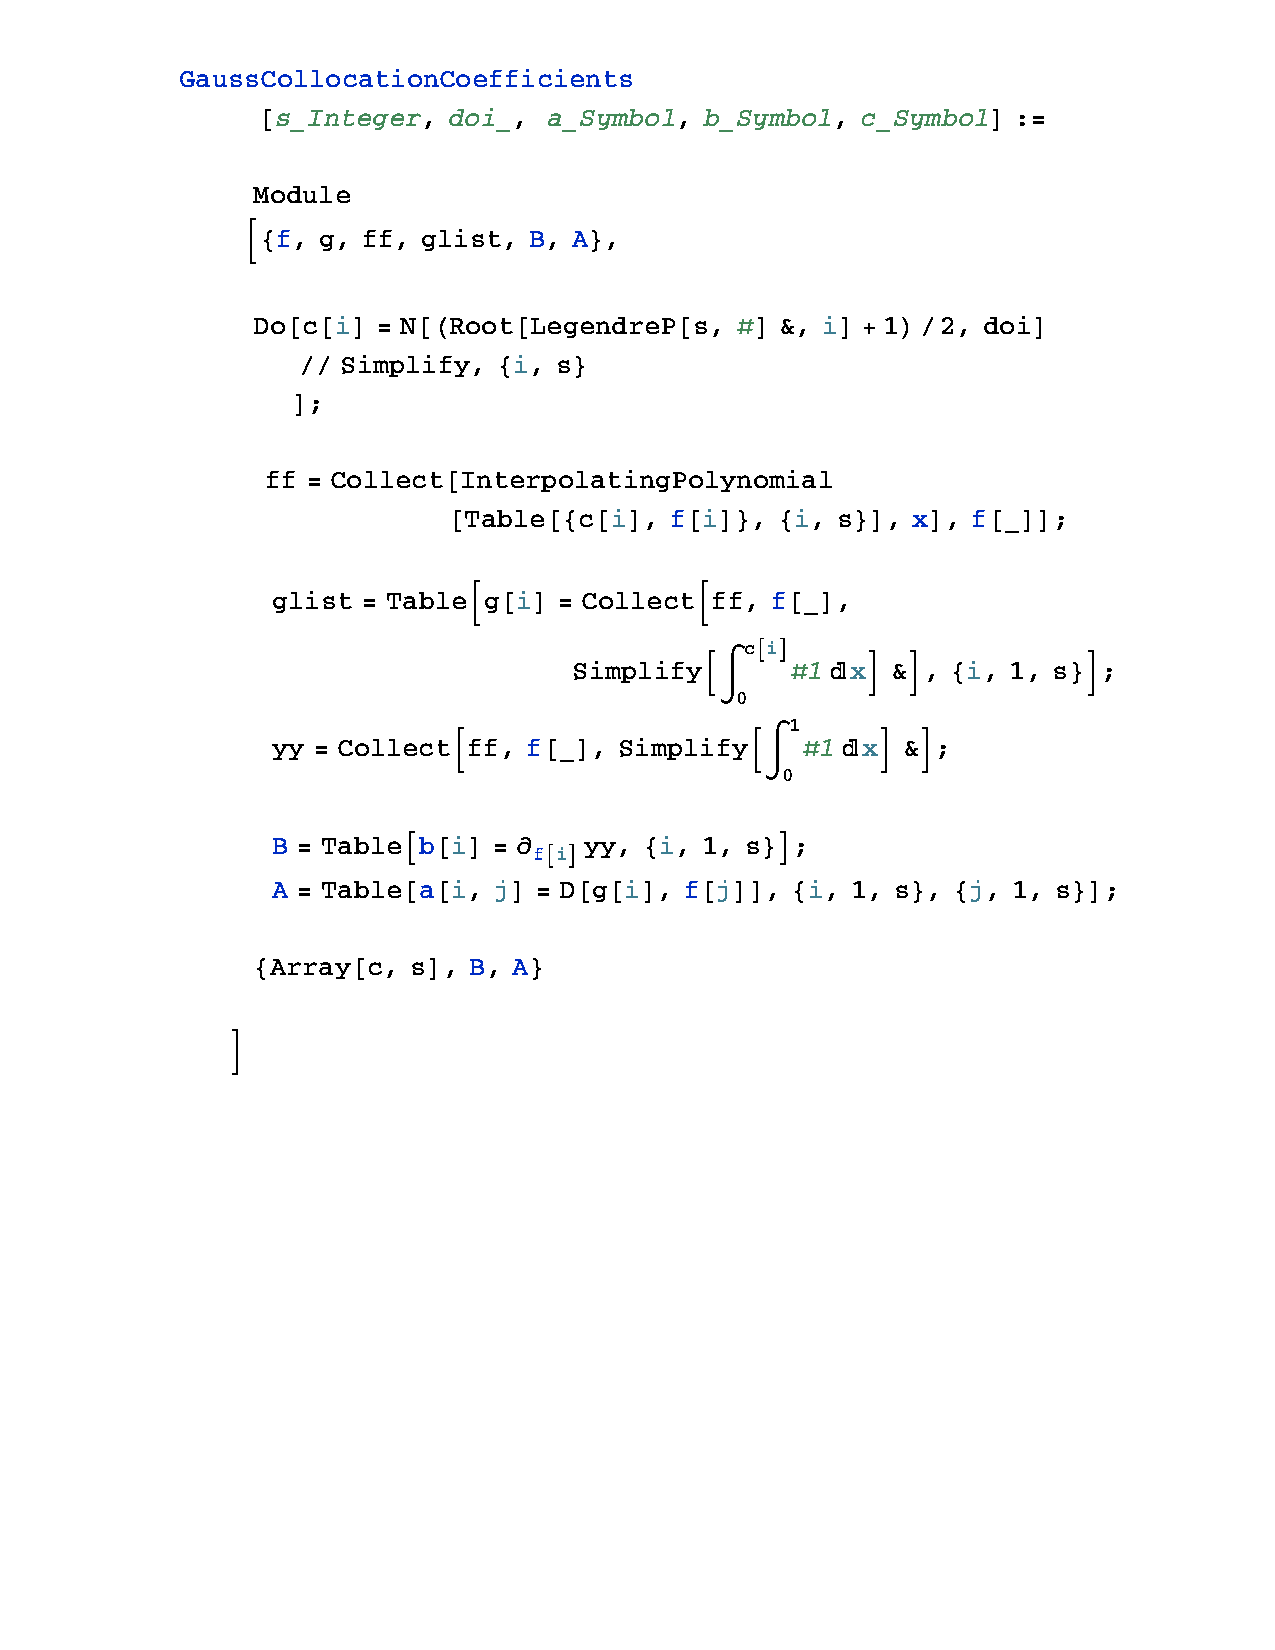
\includegraphics[width=14cm, height=18cm] {Code_Gauss}}
\caption{Code Gauss.}
\label{fig:bost}
\end{figure}

\subsection*{Atalen hasieraketa koefizienteak.}

\section{Zientzia konputazioa.}
\label{sec:C1}

\subsection*{FMA.}

Nola jakin gure \emph{linux} konputagailu batek \emph{FMA} instrukzioak dituen ala ez ? Honako agindua exekutatu eta \emph{fma} flaga azaltzen den ala ez begiratu behar dugu.
\begin{lstlisting}
$ grep fma < /proc/cpuinfo
\end{lstlisting}
eta konpilatzeko \emph{-mfma} flag-a zehaztu behar da,
\begin{lstlisting}
$ gcc -O2 -Wall -std=c99 -fno-common -mfma adibidea.c
\end{lstlisting}

\subsection*{OpenMP}

\paragraph*{\textbf{Adibidea2.}} \emph{Reduction} direktiba $+,-,*,min,max$ funtzioekin erabili daiteke. Direktiba honen adibidea emateko, trapezio erregelaren bidezko zenbakizko integrazioaren inplementazioa erakutsiko dugu.
\begin{align*}
approx=h*(f(x_0)/2+f(x_1)+f(x_2)+\dots+f(x_{n-1})+f(x_{n}))
\end{align*} 

\begin{lstlisting}[language=C]
#    include <omp.h>

     int thread_count=2;
     
     h= (b-a)/n;
     approx = (f(a)+f(b))/2.0;
     
#    pragma omp parallel for num_threads(thread_count) \
     reduction(+: approx)
      for (i = 0; i<n; i++) approx+= f(a+i*h);
      
     approx=h*approx;
\end{lstlisting}

\subsection*{Makefile adibideak.}

 
\paragraph*{Adibidea1.}
Adibide sinple baten bidez azalduko dugu bere erabilpena. Hauxe da, \emph{Makefile}-aren oinarrizko elementua,
\begin{lstlisting}
helburua: dependentziak
>TAB>  helburua lortzeko aginduak
\end{lstlisting}

Demagun aplikazioa bat hiru fitxategietan banatuta dugula,
\begin{lstlisting}[language=C]
/*file: main.c*/
void main()
{
    printf("Main program");
    sub1();
    sub2();
}
\end{lstlisting}

\begin{lstlisting}[language=C]
/*file: sub1.c*/
void sub1()
{
    printf("sub1");
}
\end{lstlisting}

\begin{lstlisting}[language=C]
/*file: sub2.c*/
void sub2()
{
    printf("sub2");
}
\end{lstlisting}

Konpilazioa automatizatzeko \emph{make} fitxategia,

\begin{lstlisting} [language=C]
main.exe: main.o sub1.o sub2.o
	      gcc main.o sub1.o sub2.o -o main.exe
main.o: main.c
        gcc -c main.c
sub1.o: sub1.c
        gcc -c sub1.c        
sub2.o: sub2.c
        gcc -c sub2.c        
\end{lstlisting}

Eta erabilpena,

\begin{lstlisting}
$ make main.exe
  gcc -c main.c
  gcc -c sub1.c
  gcc -c sub2.c
  gcc main.o sub1.o sub2.o -o main.exe
\end{lstlisting} 

\paragraph*{Adibidea2.} 
Aurreko adibidea, modu egokiagoan idatzitako \emph{make} fitxategia,

\begin{lstlisting} [language=C]

CC = /usr/bin/gcc
FLAGS=-O2 -Wall -std=c99 -fno-common 
OBJECTS=  main.o sub1.o sub2.o
.PHONY: clean help

main.exe: $(OBJECTS)
	      ${CC} $(OBJECTS) -o main.exe
	      
%.o: %.c
     ${CC} ${FLAGS} -c $<	      
	      
clean:
     rm -f $(OBJECTS) main.exe

help:
    @echo "Valid targets;"
    @echo " main.exe"
    @echo " main.o"
    @echo " sub1.o"
    @echo " sub2.o"
    @echo " clean"
             
\end{lstlisting}



\section{Problemak}

\subsection*{Pendulu bikoitza}

Mathematican,  DoublePendulum.m eta DoublePendulumSTIFF.m paketetan, hurrenez-hurren pendulu bikoitz arruntaren eta pendulu bikoitz zurrunaren honako funtzioen inplementazioak garatu ditugu:
\begin{enumerate}
   \item Hamiltondarra: DoublePendulumHam eta DoublePendulumSTIFFHam.
   \item EDA: DoublePendulumODE eta DoublePendulumSTIFFODE.
   \item Jakobiarra: DoublePendulumJAC eta DoublePendulumSTIFFJAC.
\end{enumerate}

\paragraph*{}C-lengoaiako inplementazio baliokidea, GaussUserProblem.c fitxategian inplementatu ditugu. Pendulu bikoitz arruntaren problema $problem=5$ gisa  (ode5, jac5, ham5) eta pendulu bikoitz zurrunaren problema $problem=6$ gisa (ode6, jac6, ham6) izendatu dugu.

\subsection*{N-body problema}

\paragraph*{} Mathematicako NBodyProblem.m paketean honako funtzioak garatu ditugu.

\begin{enumerate}
   \item Hamiltondarra: NBodyHAM.
   \item EDA: NBodyODE.
   \item Jakobiarra: Ez dut garatu.
\end{enumerate}

-\paragraph*{} C-lengoaiako inplementazioa:

\begin{enumerate}
   \item Hamiltondarra: HamNBody().
   \item EDA: OdeNbody().
   \item Jakobiarra: JacNBody().
\end{enumerate}

\section{Fortran kodeak}.

\paragraph*{} Haireren konposizio metodoaren Fortran kodearen  C-lengoaiako itzulpena egin dugu. Konposizio metodoaren azalpenak liburuko \cite{Hairer2006}  \emph{II.4} eta \emph{V.3} ataletan ematen dira. \emph{GNI-Comp} izeneko kodea eskuragarri dago \cite{HairerGniComp} helbidean.  

\section{IRK-Puntu finkoa}

\section{IRK-Newton}


\subsection{IRK-Newton koefizienteak.}

GaussCoefficients(s).nb mathematicako fntzioaren bidez aurrekalkulatzen ditugu koefizienteak.

\subsection{IRK-Newton eraginkorra.}

\paragraph*{} Algoritmoaren hainbat zehaztapen emango ditugu,

\begin{enumerate}

\item LAPACK.

\emph{LU deskonposaketa} egiteko funtzioa,
\begin{lstlisting} [language=C]
GETRF(LAPACK_ROW_MAJOR, n, m, MM, lda, ipiv);
\end{lstlisting}

Ekuazio sistemaren ebazpena (\emph{Solve}) egiteko,
\begin{lstlisting} [language=C]
GETRS(LAPACK_ROW_MAJOR,trans,n,nrhs,MM,lda,ipiv,fl,ldb);
\end{lstlisting}

\end{enumerate}

\section{Eguzki-sistema}

